
\chapter{Sorting}
The topic of sorting is not really specific to a data structures course, but is often used to illustrate the complexity classes of different kind of algorithms.   Sorting data is an extremely common task for computing applications and there are many  different algorithms for sorting.   Sorting algorithms are especially well researched and documented.  The internet has many high quality resources about sorting and sorting algorithms.

In general sorting algorithms assume that the data to be sorted is in a list and that the data may or may not be partially sorted.  For simplicity we will restrict the discussion to the sorting of a set of numbers in increasing order.   Sorts can easily be implemented for alphanumeric data and can place sorted elements in either increasing or decreasing order.

In this section we will briefly present six different sorting algorithms:
\begin{itemize}
\item Bubble Sort
\item Selection Sort
\item Insertion Sort
\item Shell Sort
\item Quick Sort
\item Merge Sort
\end{itemize}

For each of these sorting algorithms,  you should ensure you can answer the following questions:

\begin{enumerate}
\item What is the time complexity of the sort?  Be able to justify your answer with an analysis.
\item What is the space complexity of the sort? Be able to justify your answer with an analysis.
\item Give a 1-3 sentence summary description of the sort that distinguishes it from other sorts.
\item Identify one programming scenario for which each sort would be a good choice.
\end{enumerate}

The information provided here is only an introduction to each sorting algorithm.  Sorting is an extraordinarily well-documented topic on the internet.  There are videos, animations, tutorials,  sample programs and detailed explanations for every imaginable sort algorithm.    You are expected to ensure that you understand each  of the six sort algorithms and you may  use any resources that work for you to help you understand.   If you cannot find resources that work, please ask your instructors for help.  We'll be glad to assist you, but would like you to try to find resources on your own first, as  searching for information is an invaluable skill for computer scientists.

Finally,  there are several characteristics of sorting algorithms that are used to compare the algorithms.   As you study these sorting algorithms, ensure that you develop a definition and understanding for each of the characteristics/terms noted below.

\begin{itemize}
\item number of comparisons
\item number of swaps
\item extra memory space required for sorting
\item adaptive sort
\item in-place sort
\item divide and conquer sort
\item stable sort
\item duplicate keys
\end{itemize}

The next few subsections provide an overview for each of the six sorts we will study.  Additional resources for sorting are provided at the end of this section along with a self-test quiz.    Ensure that you can answer the self-test questions with confidence and that you can explain the answers.  It isn't enough to simply memorize the correct answers.

\section{Bubble Sort}
Bubble sort is a simple sorting algorithm and involves comparing 2 adjacent list items and swapping them if they are not in order. Bubble sort is implemented with 2 nested loops, so that for each of the "iterations" (one full loop) the next highest number is properly placed. \newline

It is not ideal for large data sets since its worst case complexity is O(n\textsuperscript{2}).\newline

Note: bubble sort can also be implemented by starting at the end of the set of data and working backwards through the list of data to sort it.

\begin{figure}[H]
\centering
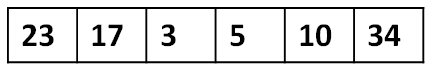
\includegraphics[width=0.5\textwidth]{pictures/bubble1.png}
\caption{Unsorted Data Set consisting of 23, 17, 3,5, 10 and 34}
\label{fig:bubble1}
\end{figure}

\begin{figure}[H]
\centering
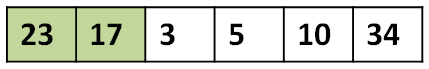
\includegraphics[width=0.5\textwidth]{pictures/bubble2.png}
\label{fig:bubble2}
\end{figure}

1\textsuperscript{st} iteration.  The final position in the list should have the correct (largest) value at the end of the iteration.  
Compare 23 and 17, a switch is needed because 23 is larger than 17.

\begin{figure}[H]
\centering
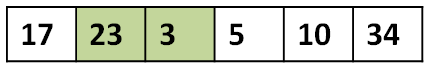
\includegraphics[width=0.5\textwidth]{pictures/bubble3.png}
\label{fig:bubble3}
\end{figure}

23 and 17 switched. Compare 23 and 3, a switch is needed.

\begin{figure}[H]
\centering
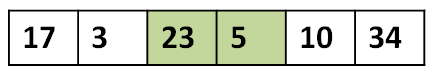
\includegraphics[width=0.5\textwidth]{pictures/bubble4.png}
\label{fig:bubble4}
\end{figure}

23 and 3 are switched. Compare 23 and 5, a switch is needed.

\begin{figure}[H]
\centering
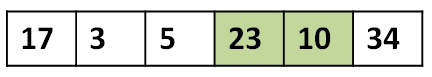
\includegraphics[width=0.5\textwidth]{pictures/bubble5.png}
\label{fig:bubble5}
\end{figure}

23 and 5 switched. Compare 23 and 10, a switch is needed.

\begin{figure}[H]
\centering
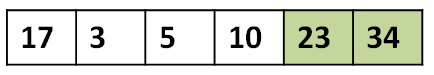
\includegraphics[width=0.5\textwidth]{pictures/bubble6.png}
\label{fig:bubble6}
\end{figure}

23 and 10 switched. Comparing 23 and 34, no switch needed. 

\begin{figure}[H]
\centering
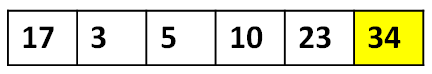
\includegraphics[width=0.5\textwidth]{pictures/bubble7.png}
\label{fig:bubble7}
\end{figure}

End of the first iteration, 34 is in the correct place.

\begin{figure}[H]
\centering
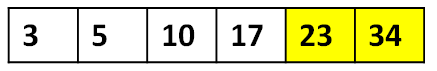
\includegraphics[width=0.5\textwidth]{pictures/bubble8.png}
\label{fig:bubble8}
\end{figure}

Intermediate steps are not shown.  End of 2\textsuperscript{nd} iteration, 23 is placed correctly.

*Note: The lower indexed places have been sorted a second time.

\begin{figure}[H]
\centering
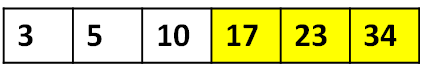
\includegraphics[width=0.5\textwidth]{pictures/bubble9.png}
\label{fig:bubble9}
\end{figure}

End of 3\textsuperscript{rd} iteration, 17 is placed correctly.

*Note: The lower indexed places have been sorted a third time even its order was already correct.

\begin{figure}[H]
\centering
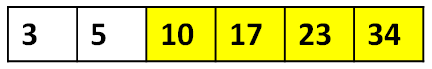
\includegraphics[width=0.5\textwidth]{pictures/bubble10.png}
\label{fig:bubble10}
\end{figure}

End of 4\textsuperscript{th} iteration, 10 is placed correctly.

\begin{figure}[H]
\centering
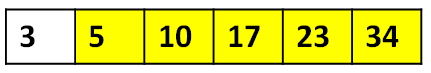
\includegraphics[width=0.5\textwidth]{pictures/bubble11.png}
\label{fig:bubble11}
\end{figure}

End of 5\textsuperscript{th} iteration, 5 is placed correctly.

\begin{figure}[H]
\centering
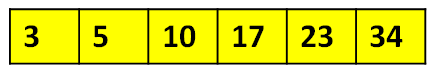
\includegraphics[width=0.5\textwidth]{pictures/bubble12.png}
\label{fig:bubble12}
\end{figure}

3 is placed correctly. No iteration should be needed for index 0, since the smallest value would have been placed correctly from the previous iteration.

\subsection{Bubble Sort Pseudocode}

\begin{lstlisting}
bubbleSort(List):List
            for(iteration: all elements in the list)
                for(i: from 0 to iteration)
                    if List[i] > List[i+1]
                        swap(List[i], List[i+1])
            return List
\end{lstlisting}

\section{Selection Sort}
Selection sort works by finding the smallest item in the data set and placing it in the smallest index. This continues n times with the sorted values being excluded from the current search. \newline

Selection sort has a worst case complexity of O(n\textsuperscript{2}) since it must to search the entire data set n times for the next smallest value. \newline

Note: selection sort can also be implemented by starting at the end of the input data, finding and placing the largest remaining value.

\begin{figure}[H]
\centering
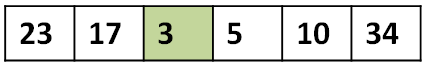
\includegraphics[width=0.5\textwidth]{pictures/selection1.png}
\caption{Unsorted Data Set consisting of 23, 17, 3,5, 10 and 34}
\label{fig:selection1}
\end{figure}

Step through the list to find the smallest value.  3 is found as the smallest value.

\begin{figure}[H]
\centering
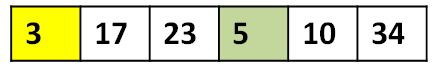
\includegraphics[width=0.5\textwidth]{pictures/selection2.png}
\label{fig:selection2}
\end{figure}

3 is placed at index 0 swapping with 23.  Search through the remaining list to find the smallest value.  5 is found as the next smallest value.

\begin{figure}[H]
\centering
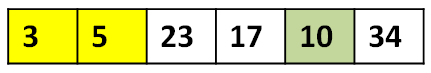
\includegraphics[width=0.5\textwidth]{pictures/selection3.png}
\label{fig:selection3}
\end{figure}

5 is placed at index 1 and 17 is placed where 5 used to be.   Step through the remaining list to find 10 as the next smallest value.

\begin{figure}[H]
\centering
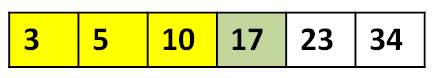
\includegraphics[width=0.5\textwidth]{pictures/selection4.png}
\label{fig:selection4}
\end{figure}

10 is placed at index 2 and 23 is place where 10 used to be. 17 is the next smallest value and it is already properly placed.

\begin{figure}[H]
\centering
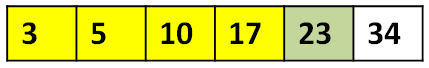
\includegraphics[width=0.5\textwidth]{pictures/selection5.png}
\label{fig:selection5}
\end{figure}

17 is left at index 3. 23 is the next smallest value and it is already properly placed.

\begin{figure}[H]
\centering
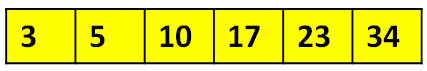
\includegraphics[width=0.5\textwidth]{pictures/selection6.png}
\label{fig:selection6}
\end{figure}

23 is left  at index 4. There is only one value left (34) which should be the largest value in the data set, no search is required for the last iteration.

\subsection{Seletion Sort Pseudocode}

\begin{lstlisting}
selectionSort(List):List
            1. Set lowestValue to index 0
            2. Search the range (lowestValue to max index) and find minimum value in the list
            3. Swap with value at location lowestValue
            4. Increment lowestValue to point to next index (shortening the search space)
            5. Repeat until list is sorted
            6. Return the List
\end{lstlisting}


\section{Insertion Sort}
Insertion sort involves designating a portion of the data list as a sorted sub-list.  The sub-list grows as the remaining list of unsorted elements shrinks, until the entire set of data resides in  the sorted sub-list. \newline

Insertion sort has a worst case complexity is O(n\textsuperscript{2}) since it needs to shuffle the data set(potentially an O(n) operation) n times to make space to add the next value to the sorted sublist. \newline

\begin{figure}[H]
\centering
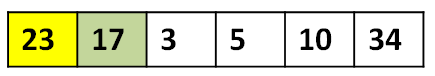
\includegraphics[width=0.5\textwidth]{pictures/insert1.png}
\caption{Unsorted Data Set consisting of 23, 17, 3,5, 10 and 34}
\label{fig:insert1}
\end{figure}

The first element is assumed to be the  sorted sub-list.   The next element (17) is examined and placed  in sorted order in the sub-list  (before 23).

\begin{figure}[H]
\centering
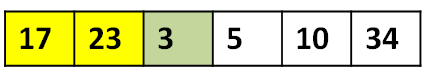
\includegraphics[width=0.5\textwidth]{pictures/insert2.png}
\label{fig:insert2}
\end{figure}

The sub-list is now 2 elements.  The next unsorted element( 3) is examined and placed in sorted order in the sub-list  (before 17).

\begin{figure}[H]
\centering
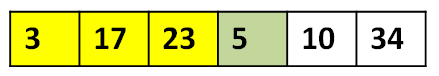
\includegraphics[width=0.5\textwidth]{pictures/insert3.png}
\label{fig:insert3}
\end{figure}

The sub-list is now 3 elements.  The next unsorted element( 5) is examined and placed in sorted order in the sub-list  (after 3).


\begin{figure}[H]
\centering
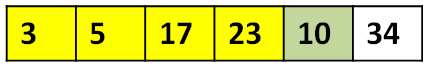
\includegraphics[width=0.5\textwidth]{pictures/insert4.png}
\label{fig:insert4}
\end{figure}

The sub-list is now 4 elements.  The next unsorted element( 10) is examined and placed in sorted order in the sub-list  (before 17).


\begin{figure}[H]
\centering
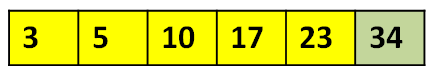
\includegraphics[width=0.5\textwidth]{pictures/insert5.png}
\label{fig:insert5}
\end{figure}

The sub-list is now 5 elements.  The next unsorted element(34) is examined and placed in sorted order in the sub-list  (after 23).


\begin{figure}[H]
\centering
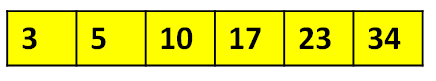
\includegraphics[width=0.5\textwidth]{pictures/insert6.png}
\label{fig:insert6}
\end{figure}

The sub-list now contains the whole list. The list is fully sorted.

\subsection{Selection Sort Pseudocode}

\begin{lstlisting}
insertionSort(List):List
            1. If it is the first element, it is already sorted. Skip to step 6
            2. Increment to next element
            3. Compare with all elements in the sorted sub-list
            4. Shift all the elements in the sorted sub-list that is greater than the value 
                to be sorted, creating an empty element
            5. Insert the value
            6. Repeat until list is sorted
            7. Return the List
\end{lstlisting}

\section{Shell Sort}

Shell sort uses a divide an conquer approach to sorting.  The initial list of data is divided into sub-lists, but the elements of the sublist are not selected sequentially from the data.   Instead the sublists are created by taking every 'kth' element from the list.

For example,  if the unsorted data were 12 5 45 6 93 10 13 2 8,  and k was set to 3,  the unsorted sublists for a shell sort would be  
\{12,6,13\}, \{5,93,2\}, \{45,10,8\}.     Each of those sublists is sorted and positioned in ascending order in the original list.  So after a 3-sort the example list would look like this

\begin{verbatim}
6 2 8 12 5 10 13 93 45
 \end{verbatim}
 
 The k-sort is then performed again, for a smaller value of k.   In this small example we could use a value of 2 for k.   The sub-lists would then be 
 \{6,8,5,13,45\} and \{2,12,10,93\}.   After sorting the data set would be in this order.
 \begin{verbatim}
6 2 5 10 8 12 13 93 45
 \end{verbatim}
 
 The last pass where k=1 is a regular insertion sort but because the data is partially ordered, the insertion sort is faster than worst case performance.


Shell sort is very efficient with a best case complexity of O(nlogn) and a worst case complexity of O(n\textsuperscript{2}).  The time complexity of shell sort depends heavily on the size of the sublists and on how the gap is changed each iteration and is often stated as near O(n) for the best case.

\begin{figure}[H]
\centering
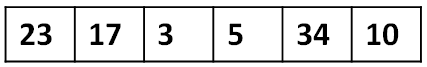
\includegraphics[width=0.5\textwidth]{pictures/shell1.png}
\label{fig:shell1}
\caption{Unsorted Data Set consisting of 23, 17, 3,5, 10 and 34}
\end{figure}

\begin{figure}[H]
\centering
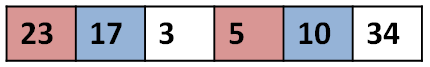
\includegraphics[width=0.5\textwidth]{pictures/shell2.png}
\label{fig:shell2}
\end{figure}

Here the sub-lists are at an interval of 3. This number is chosen based on the size of the data set.  

\begin{figure}[H]
\centering
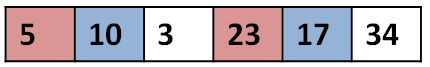
\includegraphics[width=0.5\textwidth]{pictures/shell3.png}
\label{fig:shell3}
\end{figure}

23 and 5 are compared and switched. 17 and 10 are compared and switched and 3 and 34 are compared and no switch was necessary. A total of 2 swaps were needed for the presort.

Since our interval was 3, the next step is to do an insertion sort (if our interval was greater, we would choose the next smaller interval and repeat).

\begin{figure}[H]
\centering
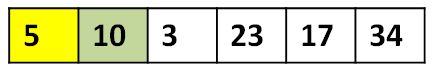
\includegraphics[width=0.5\textwidth]{pictures/shell4.png}
\label{fig:shell4}
\end{figure}

10 is inserted, no swaps were needed.

\begin{figure}[H]
\centering
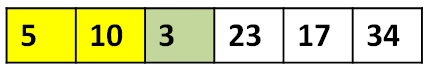
\includegraphics[width=0.5\textwidth]{pictures/shell5.png}
\label{fig:shell5}
\end{figure}

3 is inserted, 2 swaps are needed (10 and 3, then 5 and 3).

\begin{figure}[H]
\centering
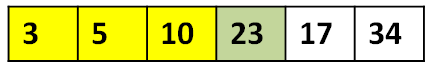
\includegraphics[width=0.5\textwidth]{pictures/shell6.png}
\label{fig:shell6}
\end{figure}

23 is inserted, no swaps were needed.

\begin{figure}[H]
\centering
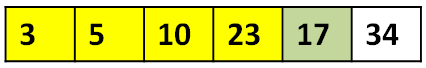
\includegraphics[width=0.5\textwidth]{pictures/shell7.png}
\label{fig:shell7}
\end{figure}

17 is inserted, 1 swap is needed.

\begin{figure}[H]
\centering
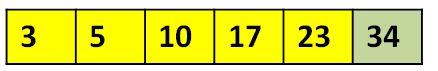
\includegraphics[width=0.5\textwidth]{pictures/shell8.png}
\label{fig:shell8}
\end{figure}

34 is inserted, no swaps were needed.

\begin{figure}[H]
\centering
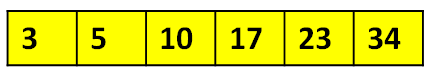
\includegraphics[width=0.5\textwidth]{pictures/shell9.png}
\label{fig:shell9}
\end{figure}

In total shell sort involved 5 swaps. In order to sort the same data set by just insertion sort 7 swaps are needed. As the data sets get larger, the difference between the number of swaps increases.

\subsection{Shell Sort Pseudocode}

\begin{lstlisting}
shellSort(List):List
	Do until the gap size is 1
            Divide the list into sub-lists using the gap size 
            Sort the sub-lists(in place) using insertion sort
	 Use insertion sort on the whole list

\end{lstlisting}


\section{Quick Sort}
Quick sort works by dividing the data set and sorting the  resulting segments recursively. 
A pivot point is selected to divide the data set.  The pivot point can be any position in the list of data.  Sometimes the last position is selected, sometimes the first,  often the middle position in the list is selected.   Any values smaller than the value at the  pivot  point are placed on the left side of the pivot.  All the elements with values greater than the value at the pivot point are placed to the right of the pivot.

The problem is then reduced, by recursion to sorting the two segments independently.   The elements on the left side of the pivot are sorted via quicksort as if they were an independent data set, as are the values on the right side of the pivot.   The algorithm recurses until each segment is 2 elements, which results in a sorted list.   When all recursive calls have returned,  the elements will be sorted.



Quick sort has a worst case complexity of O(n\textsuperscript{2}). More typically has a complexity of O(nlog(n)) when for each iteration the pivot value is at approximately the middle (value) of the data set.    The choice of pivot point has a significant impact on the complexity of quick sort.

Recursive sorts are more easily visualized using a larger set of data than we've used for our previous examples.  




\begin{figure}[H]
\centering
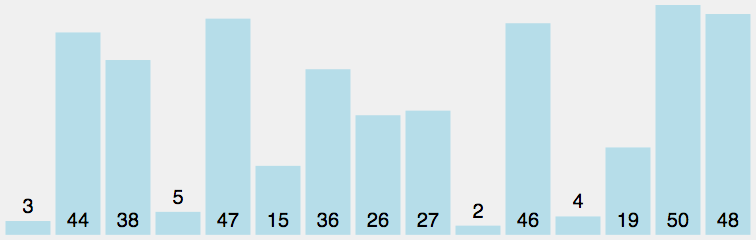
\includegraphics[width=0.5\textwidth]{pictures/quick1.png}
\label{fig:quick1}
\caption{Unsorted Data Set: 3, 44, 38, 5, 47, 15, 36, 26, 27, 2, 46, 4, 19, 50, 48}
\end{figure}

\begin{figure}[H]
\centering
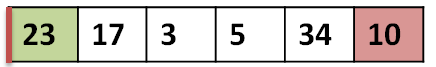
\includegraphics[width=0.5\textwidth]{pictures/quick2.png}
\label{fig:quick2}
\end{figure}

Select the first element as the pivot (3).  For each element  to the right of the pivot, move the element to the left of the pivot if it is less than the pivot value.
 

\begin{figure}[H]
\centering
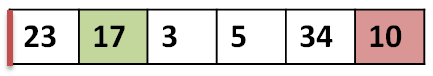
\includegraphics[width=0.5\textwidth]{pictures/quick3.png}
\label{fig:quick3}
\end{figure}

We now have two unsorted partitions, one to the left of the pivot and one to the right.  We know that the pivot value is in the correct position.  
We repeat the sort on the two partions.   The single element to the right of the pivot is already sorted, so there is no work to do there.
We select a new pivot (38) from the partition to the right of 3.
For each element to the right of 38, move the element to the left of 38 if it is less than 38.


\begin{figure}[H]
\centering
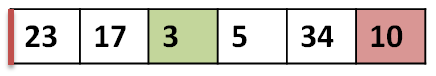
\includegraphics[width=0.5\textwidth]{pictures/quick4.png}
\label{fig:quick4}
\end{figure}

We now have three partitions  and one pivot in the original data.  We have the sorted partition consisting of 2,3.   We have an unsorted partition to the left of 38 consisting of 19, 5, 15, 36, 26, 27, 4 and an unsorted partition to the right of 38 consisting of 46, 47, 44, 50, 48.   

The recursive process continues until the unsorted partitions are ,  working through the two unsorted partitions using the same  procedure of selecting a pivot and placing the elements on either side of the pivot.    Once all of the partitions have reached the size of 2 or 1, the elements in the entire array will be sorted.



\begin{figure}[H]
\centering
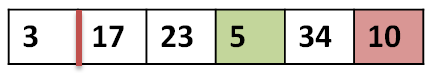
\includegraphics[width=0.5\textwidth]{pictures/quick5.png}
\label{fig:quick5}
\end{figure}

The first 6 elements of the list are known to be sorted at this point (2,3,4,5,15,19) and the algorithm is working on the partition to the right of 26.

%\begin{figure}[H]
%\centering
%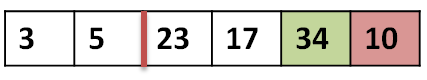
\includegraphics[width=0.5\textwidth]{pictures/quick6.png}
%\label{fig:quick6}
%\end{figure}

Quick sort is most easily understood by watching a dynamic illustration.  Please use one of the additional resources given at the end of this section to observe the quicksort in action.  The images used to illustrate quicksort were generated using \url{https://visualgo.net/en/sorting}

\subsection{Quick Sort Pseudocode}

\begin{lstlisting}
quickSort(List, pivotIndex, startIndex):List
            1. Select a pivot (simple case is to select the first element in the partion
            2. Partition the list using pivot value by putting all elements greater than the pivot to the right of the pivot and all elements less than the pivot to the left of the pivot.
            3. Quick sort left partition recursively
            4. Quick sort right partition recursively
            7. Return the List
\end{lstlisting}

\section{Merge Sort}

Merge sort is another recursive sort. It works be dividing the data set in half and recursively calling the sort on each half.  The recursive base case is invoked when the sub-set of data  can no longer be divided.  On the return from the recursion the lists are merged in sorted order. 

Merge sort is  consistent sorting algorithm as it has a worst case complexity of O(nlog(n)). 

Note: Each colour represents a sub-list

\begin{figure}[H]
\centering
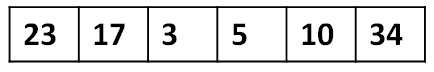
\includegraphics[width=0.5\textwidth]{pictures/merge1.png}
\label{fig:merge1}
\caption{Unsorted Data Set}
\end{figure}

\begin{figure}[H]
\centering
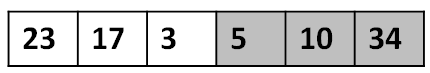
\includegraphics[width=0.5\textwidth]{pictures/merge2.png}
\label{fig:merge2}
\end{figure}

The data set is split into 2 sub-lists of length 3.

\begin{figure}[H]
\centering
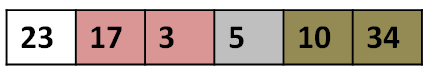
\includegraphics[width=0.5\textwidth]{pictures/merge3.png}
\label{fig:merge3}
\end{figure}

Each sub-lists is  split into 2 sub-lists (one of length len/2 and one of length (len/2 + len\%2)). 

\begin{figure}[H]
\centering
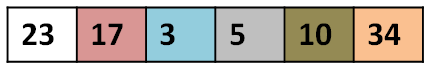
\includegraphics[width=0.5\textwidth]{pictures/merge4.png}
\label{fig:merge4}
\end{figure}

The sub-lists containing 23 and 5 can not be divided again. The remaining sub-lists are split again.

\begin{figure}[H]
\centering
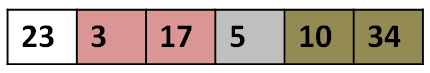
\includegraphics[width=0.5\textwidth]{pictures/merge5.png}
\label{fig:merge5}
\end{figure}

The algorithm begins the return out of the recursion.  The sub-lists containing 3 and 17 are sorted and combined into a single list. 10 and 34 are likewise combined into a single list.

\begin{figure}[H]
\centering
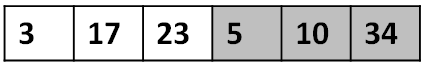
\includegraphics[width=0.5\textwidth]{pictures/merge6.png}
\label{fig:merge6}
\end{figure}

23 is  combined with 3 and 17.  5 is combined with 10 and 34.

\begin{figure}[H]
\centering
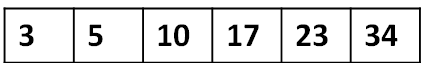
\includegraphics[width=0.5\textwidth]{pictures/merge7.png}
\label{fig:merge7}
\end{figure}

The 2 original sub-lists are now sorted and are merged to produce a sorted list.

\subsection{Merge Sort Pseudocode}

\begin{lstlisting}
mergeSort(List):List
            1. Check length of the list, if it is only one element it is already sorted, 
                skip to step 6
            2. Divide the list by 2 (one partition is len/2, the other would be (len/2 + len\%2). 
                This accounts for numbers not divisible by 2) 
            3. Merge sort left partition recursively
            4. Merge sort right partition recursively
            5. Merge the smaller lists into new list in sorted order.
            6. Return the list
\end{lstlisting}

The hardest step in a merge sort is the merging of two sorted lists.  The merge step is accomplished by identifying the smallest element, then the next smallest, making swaps as necessary to put them in order.  A single merge step is an O(n) operation since both sublists are sorted.

\section{Additional Resources}

\begin{itemize}
\item \url{https://visualgo.net/en/sorting?}
\item \url{https://www.tutorialspoint.com/data_structures_algorithms/sorting_algorithms.htm}
\item \url{https://www.youtube.com/channel/UCIqiLefbVHsOAXDAxQJH7Xw}
\item \url{https://www.toptal.com/developers/sorting-algorithms/}
\item \url{https://en.wikipedia.org/wiki/Sorting_algorithm}
\item \url{https://www.youtube.com/watch?v=kPRA0W1kECg}
\item \url{http://bigocheatsheet.com/}

\end{itemize}

\section{Self-Test Questions}

\begin{verbatim}

 Which of the following statements is true about Insertion Sort? 

*a. It is a comparison Sort 
*b. It is an adaptive Sort

c. It has O(nlogn) complexity for the best case. 
*d. It has O(n-squared) complexity for the worst case 
e. It performs more comparisons than Selection Sort 
f. It is always outperformed by divide and conquer sorts 
*g. It requires O(1) extra memory 
*h. It is an in-place sort. 





Which of the following scenarios might be a good situation in which to use insertion sort? 

a. When only alphabetical sort is required. 
b. When you are sorting more than 20 items. 
*c. When you are sorting fewer than 20 items 
*d. When you have very little extra memory space 
e. When you need an extremely fast sort 
*f. When the comparison operator is computationally expensive 
*g. When the list must be sorted as the data is generated, one item at a time 
h. When only large numbers will be sorted 


Which part of the algorithm for insertion sort causes the average case running time? 

a. The assignment of different values into the temporary variable. 
b. The loop that goes through the array one element at a time. 
*c. The nested loops that each go through the array one element at a time. 
d. The multiple places where the boolean variable finished is assigned a value. 


Which of the following statements are true about Selection Sort? 

*a. It is O(n squared) for the average case 
b. It is an adaptive sort. 
*c. It requires fewer swaps than many algorithms. 
*d. It generally performs worse than insertion sort. 
*e. It is sometimes faster than a divide and conquer algorithm. 
f. It is not an in-place sorting algorithm. 
*g. It is similar to a heapsort. 
*h. It can be written to be a stable sort. 




Which of the following scenarios might be a good situation in which to use selection sort? 

*a. When you are sorting 20 items or fewer 
b. When you are sorting more than 20 items 
c. When you know that your data will be partially sorted. 
*d. When the algorithm for swapping data values is computationally expensive. 
e. When the data to be sorted is in a linked list. 
*f. When you must minimize the amount of auxillary memory used. 
g. When you are sorting a set of complex data structures 
h. When your data must be sorted twice, such as by last name and then age. 


Selection sort has the same computational cost for worst, average and best cases. Which statement below best describes why this is so? 

a. Because comparisons are only made outside the inner loop. 
*b. Because the number of times through the loops is not influenced by the values in the array. 
c. Because the sort must go through the array of values the same number of times no matter what the data is. 
d. Because it swaps the values rather than storing one value in a temporary location. 


Which of the following statements are true about Shell Sort?
a. The solution is recursive.
*b. Shell sort is an unstable sort.
*c. Shell sort is an in-place sort.
d. Shell sort is always more efficient than Merge Sort.
*e. The time complexity of Shell sort is dependent on the increment sequence of the gaps.



Which of the following statements are true about Merge Sort? 

*a. The solution can use recursion 
*b. The worst case complexity is O(nLogn) 
c. It is not a stable sort 
d. It is adaptive 
*e. It is similar to a binary tree sort 
*f. It works well when sorting structures that do not permit random access (linked lists) 
g. It is difficult to write a parallel version. 
h. Is worse than quicksort (running time, number of comparisons, memory used, and number of writes) 





Merge sort has a running time of O(n log n) for worst and average cases. Which of the following statements adds correct details to the description of merge sort's running time? 

*a. The number of comparisons merge sort makes is O(log2 n) 
*b. Merge sort requires 2n auxillary space 
*c. Merge sort makes O(n) recursive calls 
d. Merge sort can be written as a non recursive sort 


Which of the following scenarios might be a good situation in which to use a merge sort? 

*a. When your sorting must be stable 
b. When you know the data will be partially sorted. 
*c. When you need to use the sort on data that is on a tape drive 
*d. When you need the sort to have the same running time, no matter what the data is. 
*e. When you have a lot of data to sort. 


Which of the following statements are true about Quick Sort? 

a. It is a stable sort. 
*b. It can be implemented as in in-place sort. 
*c. It can be implemented recursively. 
*d. It is O(n log n) for the average case. 
e. The worst case running time is the same as the average case. 
f. It is an adaptive sort. 




Which of the following scenarios might be good situation in which to use quick sort? 

a. When you know that your data is going to be partially sorted. 
*b. When the order of duplicate keys in your data does not matter. 
c. When you must guarantee no more than nLogn running time. 
*d. When the amount of memory available is limited. 
*e. When the amount of data to be sorted is large. 
f. When all the data to be sorted must be encrypted. 

\end{verbatim}
